\label{Sec:Methods}
\subsection{Reservoir modeling of deep carbon}

In order to model the time evolution of carbon cycle in the case that the source of carbon in the continetnal crust is the atmosphere (Model A-CC), we construct a simplified reservoir model which includes three reservoirs: the atmosphere, continental crust and the mantle. A list of symbols used to describe the reservoir model is shown in Table.~\ref{Table:List of Symbols} and a flow diagram of the reservoir model is shown in Fig.~\ref{Fig:ReservoirFlowDiagram}.

\begin{table}[h!]
    \centering
    \caption{A list of symbols used in this paper.}
    \scalebox{1.0}{
    \begin{tabular}{lllll}
        \hline
        Symbol       & Quantity                                             & Unit    & Model A-CC   & Model M-CC \\
        \hline
        $t$          &Time                                                  & Ga   & $t_0 < t < t_p$ & $t_0 < t < t_p$ \\
        $t_0$        &Initial time starting post giant-moon forming impact  & Ga   & 4.4 & 4.4   \\ 
        $t_{cc0}$    &Starting time of continental crust formation          & Ma   & 500  & 500 \\   
        $t_p$        &Present time                                          & Ga   & 0 & 0  \\
        $\tau_{acc}$ &Time constant for Urey reaction                       & Ga   & 1 &  1 \\
        $\tau_{am}$  &Time constant for loss of carbon from atm. to mantle  & Ma   & 20 &  -  \\
        \mass{a}$(t_0)$  & Initial mass of carbon in the atmosphere         & Gt   & $1.57 \times 10^8$ & $0$ \\
        \mass{m}$(t_p)$  & Present mass of carbon in the mantle~\citep{KLH-TDL-WM:2018}           & Gt   & $2 \times 10^8$ & $2 \times 10^8$ \\
        \mass{cc}$(t_p)$ & Present mass of carbon in the continental crust~\citep{KHW:1995}  & Gt   & $4.2 \times 10^7$ & $4.2 \times 10^7$ \\
        \mass{a}$(t_p)$ & Present mass of carbon in the atmosphere~\citep{NOAA:2017}          & Gt   & $8.5 \times 10^2$ & $8.5 \times 10^2$ \\
        \cflux{a}{m} &Flux of carbon from atm. to mantle                     & Mt/yr  & & - \\
        \cflux{a}{cc} &Flux of carbon due to Urey reaction                   & Mt/yr  & & \\
        \cflux{cc}{a} &Flux of carbon due to island arc volcanism            & Mt/yr  & & \\
        \cflux{cc}{m} &Flux of carbon due to subduction                      & Mt/yr  & & \\
        \cflux{m}{a}  &Flux of carbon due to mid-ocean ridge volcanism       & Mt/yr  & & \\
        \hline
    \end{tabular}
               }
    \label{Table:List of Symbols}
\end{table}


The time period of interest is post core crystallization, $t_0$ to present time, $t_p$. Let $t_{cc0}$ be the time at which continental crust formation began. ~\citet{SNH-ZK:2001} hypothesized that from $t_0 \le t \le t_{cc0}$, due to the giant-moon forming impact, the resulting solid surface crust of global magma ocean absorbed a significant portion of carbon from the atmosphere. Episodic foundering of this dense crust transported carbon into Earth's mantle ~\citep{KLH-TDL-WM:2018}. Once the magma ocean cooled down and solidified, we hypothesize that the remaining carbon in the atmosphere became the source of carbon in the continental crust through the Urey reaction.

In testing this hypothesis, the following ODE system for the time evolution of carbon in the three reservoirs is defined from $t_0 \le t \le t_{cc0}$, 

\begin{align}
  \frac{d\,\mass{a}}{dt} &= -\,\cflux{a}{m} \\
  \frac{d\,\mass{cc}}{dt} &= 0 \\
  \frac{d\,\mass{m}}{dt} &= \cflux{a}{m}.
\end{align}

\noindent where $\cflux{a}{m} = -\frac{\mass{a}}{\tau_{am}}$.
 
From $t_{cc0} \le t \le t_p$, the time evolution of carbon in the three reservoirs is

\begin{align}
  \frac{d\,\mass{a}}{dt} &= -\,\cflux{a}{cc} + \cflux{m}{a} + \cflux{cc}{a}\\
  \frac{d\,\mass{cc}}{dt} &= \cflux{a}{cc} - \cflux{cc}{m} - \cflux{cc}{a}\\
  \frac{d\,\mass{m}}{dt} &= -\,\cflux{m}{a} + \cflux{cc}{m}.
\end{align}

where $\cflux{a}{cc} = -\frac{\mass{a}}{\tau_{acc}}$, and the remaining fluxes are approximated as exponential functions. For example, $\cflux{m}{a}(t) = \frac{\mass{m}}{\mass{m}(t_p)}\, \cflux{m}{a}(t_p) \exp((t_p - t)/t_{cc0})$. Then by specifying the abundance of carbon in the three reservoirs at present time, which are shown in Table.~\ref{Table:List of Symbols} and present fluxes between the reservoirs, the ODE system can be solved. The solution is shown in Fig.~\ref{Fig:ModelA-CC}. Note that the fluxes between reservoirs are time-dependent. 

%{\renewcommand{\arraystretch}{2.0}% for the vertical padding
%\begin{table}[h!]
%    \centering
%    \begin{tabular}{|l|l|l|c|c|}
%        \hline
%        Reservoir & Symbol & Mass of carbon Gt & Reference \\
%        \hline
%        Core   & \mass{c} & $4 \times 10^9$ & ~\citet{DR:2013}  \\
%        \hline
%        Mantle & \mass{m} & $2 \times 10^8$ & ~\citet{KLH-TDL-WM:2018}  \\
%        \hline
%        Continental crust & \mass{cc} & $4.2 \times 10^7$ & ~\citet{KHW:1995} \\
%        \hline
%        Oceans & \mass{o} & $3.8 \times 10^4$ & ~\citet{HRA:2007} \\
%        \hline
%        Atmosphere & \mass{a} & $8.5 \times 10^2$ & ~\citet{NOAA:2017} \\
%        \hline
%        Total & & $4.24 \times 10^9$ & \\
%        \hline
%    \end{tabular}
%    \caption{\doublespacing Masses of carbon in the Earth's carbon reservoirs (1 Gt $= 10^{12}$ kg) ~\cite{KLH-TDL-WM:2018}.
%    }
%    \label{Table:Masses of carbon in Earth's reservoirs}
%\end{table}

\begin{figure}[h!]
  \centering
  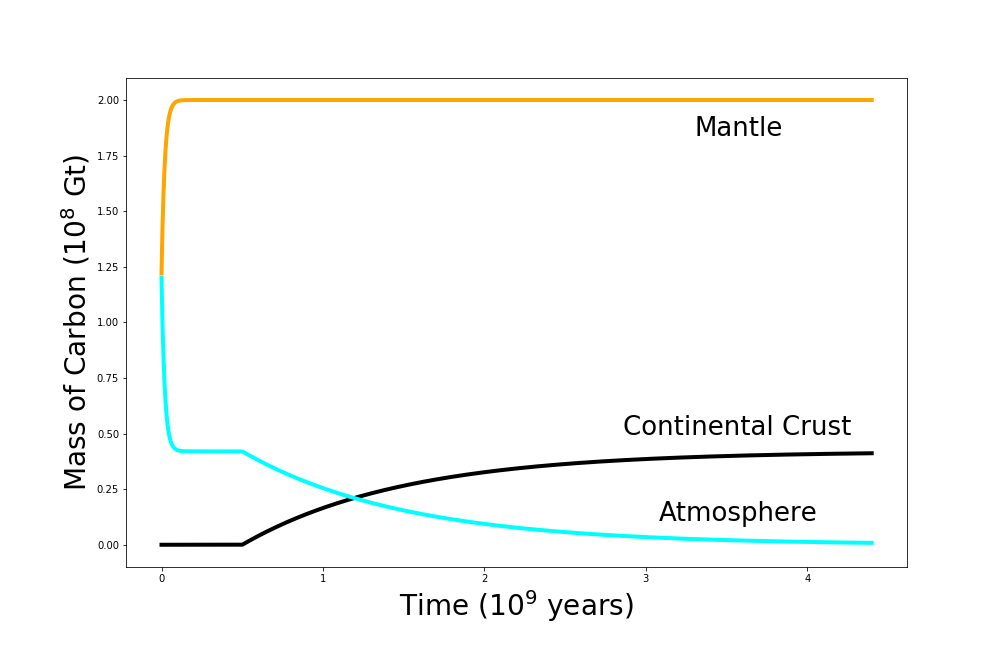
\includegraphics[scale=0.4]{Figures/ModelM-CC.png}
  \caption{Preliminary results of the time evolution of carbon cycle in Model A-CC where the source of carbon in the continental crust is the mantle.}
  \label{Fig:ModelA-CC}
\end{figure}

Since from time, $t_{cc0}$ onwards, the influx of carbon due to subduction is equal to the outflux of carbon due to volcanism, the mass of carbon in the mantle remains constant in Model A-CC. If however, the carbon flux due to volcanism is greater than the carbon flux due to subduction, the source of carbon in the continental crust is the mantle (Model M-CC). The same system of ODE can be assembled and solved for Model M-CC where $\tau_{am} = 0$, $\cflux{cc}{m} < \, \cflux{m}{a}$, and \mass{a}$(t_0) = 0$ Gt.

%\begin{figure}[h!]
%  \centering
%  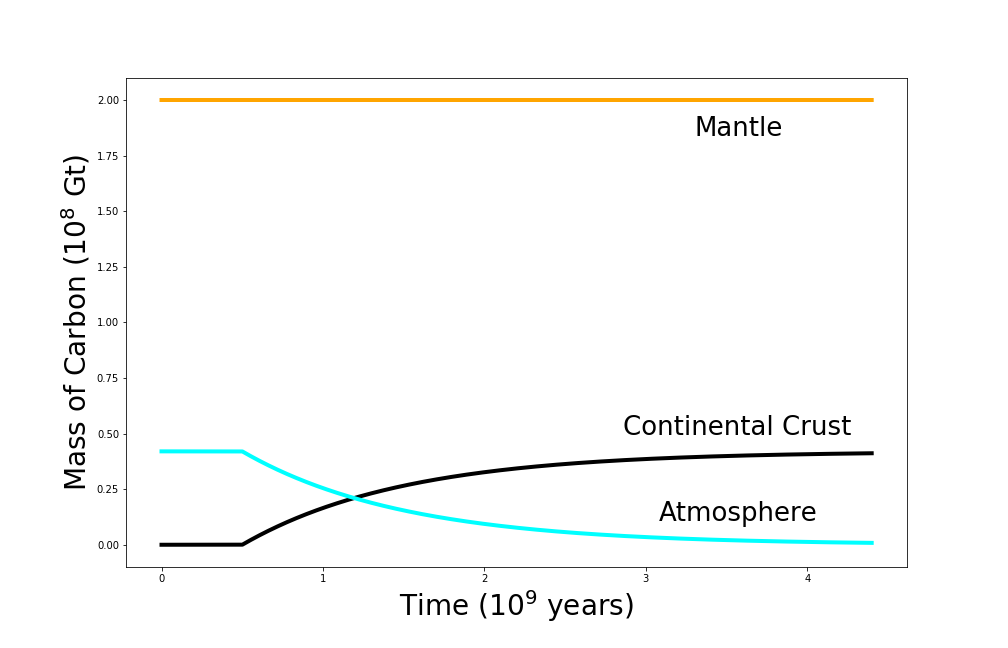
\includegraphics[scale=0.4]{Figures/ModelA-CC.png}
%  \caption{Preliminary results of the time evolution of carbon cycle in Model A-CC where the source of carbon in the continental crust is the atmosphere.}
%  \label{Fig:ModelA-CC}
%\end{figure}

A combination of the two limiting cases described above is also plausible. By introducing an independent parameter, we can then control what portion of the source of carbon in the continental crust is attributed to the atmosphere or mantle.

\subsection{Designing a reservoir modeling library in python}

Let a reservoir model $G = (R, E)$ be represented as a directed graph consisting of a set of reservoirs, $r_1, r_2, ..., r_{n} \in R$ such that $n \in \mathbb{N}$ and a set of edges, $e_1, e_2, ..., e_n \in E$ such that $n \in \mathbb{N}$. If $(r_1,r_2) \in E$ represents an edge from reservoir $r_1$ to reservoir $r_2$, then we can define a flux function, \flux{r_1}{r_2}. For a given reservoir $r_m$, the outflux vector is

\begin{equation}
\renewcommand\arraystretch{0.5}
\vec{J}^{o}(r_m) = 
\begin{bmatrix}
    \flux{r_m}{r_1} \\
    \flux{r_m}{r_2} \\
    \vdots \\
    \flux{r_m}{r_m} \\
    \vdots \\
    \flux{r_m}{r_n}
\end{bmatrix}
\end{equation}

and the influx vector is

\begin{equation}
\vec{J}^{i}(r_m) =
\renewcommand\arraystretch{0.5}
\begin{bmatrix}
    \flux{r_1}{r_m} \\
    \flux{r_2}{r_m} \\
    \vdots \\
    \flux{r_m}{r_m} \\
    \vdots \\
    \flux{r_n}{r_m}.
\end{bmatrix}
\end{equation}

By treating a reservoir model as a directed graph, we can use adjacency matrix, $A$ to represent the set of reservoirs and pathways in the model. Fig.~\ref{Fig:DG-AdjMatrix} shows an example reservoir model and its adjacency matrix representation ~\citep{CTH:2009}. For an arbitrary number of reservoirs, $A$ will be an n by n matrix. For a given reservoir, $r_m$, the row vector $A_m$ represents the outgoing fluxes from reservoir $r_m$ to all other reservoirs and a row vector of $A^{T}_{m}$ then represents the incoming fluxes from all other reservoirs to $r_m$. We can then assemble the following system of ordinary differential equations (ODEs) as

\begin{equation}
\renewcommand\arraystretch{1.0}
\begin{bmatrix}
    r_1' \\
    r_2' \\
    \vdots \\
    r_n'
\end{bmatrix}
=
\renewcommand\arraystretch{1.0}
\begin{bmatrix}
    A^T_1\vec{J}^{i}(r_1) - A_1\vec{J}^{o}(r_1) \\
    A^T_2\vec{J}^{i}(r_2) - A_2\vec{J}^{o}(r_2) \\
    \vdots  \\
    A^T_n\vec{J}^{i}(r_n) - A_n\vec{J}^{o}(r_n) \\
\end{bmatrix}
=
\renewcommand\arraystretch{1.0}
\begin{bmatrix}
    \sum_{i=1}^n \flux{r_i}{r_1} - \sum_{i=1}^n \flux{r_1}{r_i} \\
    \sum_{i=1}^n \flux{r_i}{r_2} - \sum_{i=1}^n \flux{r_2}{r_i} \\
    \vdots  \\
    \sum_{i=1}^n \flux{r_i}{r_n} - \sum_{i=1}^n \flux{r_n}{r_i}
\end{bmatrix}
\end{equation}

\noindent Given initial conditions, the system of ordinary differential equations (ODEs) can then be solved for using available ODE solvers in Python.

\begin{figure}[h!]
  \centering
  \begin{subfigure}[b]{0.49\textwidth}
    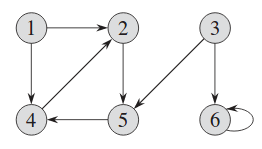
\includegraphics[width=0.49\textwidth]{Figures/directedGraphDiagram.png}
    %\caption{A directed graph G.}
    %\label{Fig:DirectedGraph}
  \end{subfigure}
  \begin{subfigure}[b]{0.49\textwidth}
    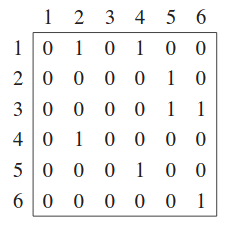
\includegraphics[width=0.49\textwidth]{Figures/adjMatrix.png}
    %\caption{Adjacency-matrix representation of G}
    %\label{Fig:AdjMatrix}
  \end{subfigure}
  \caption{Left is an example reservoir model and its adjacency-matrix representation is shown on the right.} 
  \label{Fig:DG-AdjMatrix}
\end{figure}

